\newpage
\section{Entwurf und Aufbau der Datensammlungsumgebung}
TBD

\subsection{Integration diverser Datenströme in einem einheitlichen Datenkorpus}
Die erste Datenquelle für die Datensammlungsumgebung ist die Anwendungsschnittstelle der Tagesschau. Diese ist eine Nachrichtensendung der Arbeitsgemeinschaft der öffentlich-rechtlichen Rundfunkanstalten der Bundesrepublik Deutschland (ARD) . Über diese Schnittstelle ist es möglich, Beiträge der Website www.tagesschau.de im JavaScript Object Notation (JSON) Format abzufragen. Der Zugriff auf diese Schnittstelle ist auf 60 Aufrufe pro Stunde limitiert. Darüber hinaus ist lediglich die nicht-kommerzielle Nutzung gestattet. Zudem dürfen gesammelte Inhalte, mit Ausnahme der unter der Creative Common (CC) Lizenz stehenden Inhalte, nicht weiter veröffentlicht werden. \footcite [Vgl.][]{TagesschauAPI}

Die Schnittstelle gruppiert sich in 4 Themensegmente, welche über eigene Endpunkte verfügen. 
\begin{itemize}
    \item Homepage - Abfrage von Nachrichten und Eilmeldungen der Startseite
    \item News - Abfrage von sämtlichen Nachrichten und Eilmeldungen
    \item Channels - Abfrage von Kanälen
    \item Search - Allgemeine Suche über alle Inhalte der Plattform
\end{itemize}
Jeder Endpunkt ist gemäß dem Paradigma Representational State Transfer (REST) konstruiert und wird entsprechend über das Hypertext Transfer Protocol (HTTP) abgefragt. \footcite [Vgl.][]{TagesschauAPI}

Für die erste Umsetzung der Datensammlungsumgebung ist es ausreichend, den News Endpunkt zu konsumieren. Dieser gibt eine Liste von News Objekten zurück, wie im \ref{Anhang} beschrieben. Diese enthalten folgende Informationen:
\begin{itemize}
    \item news - Bildet das Hauptelement , welches die verschiedenen Nachrichten enthält
    \item sophoraId - Eindeutige Identifikationsnummer 
    \item externalId - Zusätzliche eindeutige Identifikationsnummer
    \item title - Titel der Nachricht
    \item teaserImage - Enthält Informationen über das Vorschaubild der Nachricht
    \item date - Das Veröffentlichungsdatum des Artikels
    \item tracking - Liste von Objekten, welche Tracking-Informationen beinhalten
    \begin{itemize}
        \item sid - Session Id zum Nachverfolgen des Nutzerverhaltens
        \item src - Quelle des Artikels, zeigt z.B. auf den Kanal, aus welchem der Artikel stammt
        \item ctp - Art des Inhaltes als technischer Kenner
        \item pdt - Datum der Veröffentlichung (eng. Publish Date Time)
        \item otp - Art des Inhaltes als fachlicher Kenner, z.B. \textit{meldung} 
        \item cid - Eindeutige Identifikationsnummer
        \item pti - Titel der Seite (eng. Page Title)
        \item pcr - Flaggen Attribut, Verwendung ist unbekannt
        \item type - Typ des Tracking Objektes, z.B. \textit{generic}
    \end{itemize}
    \item tags - Liste von Objekten, welche Schlagwörter enthalten
    \item updateCheckUrl  - Adresse zur Überprüfung von Aktualisierungen der Nachricht
    \item  regionId - Identifikationsnummer, welche den regionalen Bezug der Nachricht angibt
    \item details - Adresse zum Abfragen des Artikels im JSON Format
    \item detailsweb -  Adresse zum Abfragen des Artikels im HTTP Format
    \item shareURL  -  Adresse zum Artikel zum Teilen der Nachricht über soziale Medien
    \item topline  - Kurze Zusammenfassung der Nachricht
    \item firstSentence  - Erster Satz der Nachricht
    \item geotags - Enhält eine Liste von Objekten, welche die geographischen Informationen des Artikels beinhalten
    \item type - Typ der Nachrichtenseite, z.B. \textit{news page}
    \item nextPage - Adresse auf die nächste Seite mit weiteren Nachrichten
    \item comments - Adresse zur Kommentarsektion eines Artikels, sofern vorhanden
    \item ressort - Themenfeld des Artikels, z.B. \textit{ausland}
    \item breakingNews - Boolescher Wert, ob der Artikel als Eilmeldung veröffentlicht wurde
\end{itemize}

Die erste Ebene der Datenstruktur enthält primär Metadaten zu einer Nachricht. Um den, für die Sammlung relevanten, Inhalt zu erhalten, sind die Referenzen auf die Details sowie die Kommentare aufzulösen. 
Die darauf folgende Antwort ist 


Der zu erstellende Datenkorpus vereinigt alle, für die Analyse relevanten, Daten der verschiedenen Datenquellen miteinander.

\newpage
\subsection{Architektur und Design der Datensammlungsumgebung}

Um das Limit der Tagesschau API von 40 Anfragen pro Stunde nicht zu überschreiten, wurde folgender Batch Job konzipiert. 

\begin{figure}
    \centering
    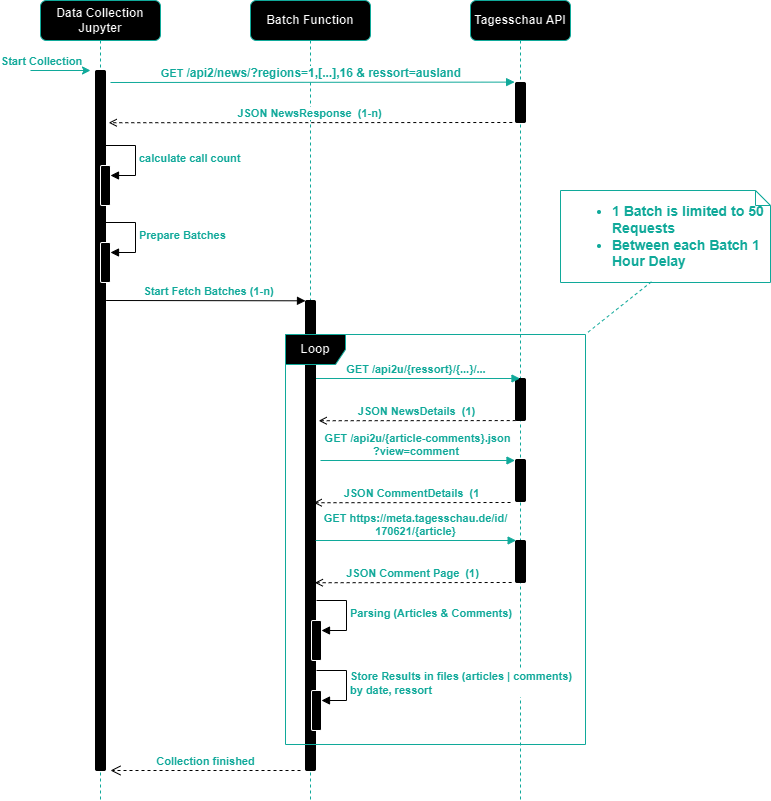
\includegraphics[width=1\linewidth]{abbildungen/image.png}
    \caption{Sequenzdiagramm Abfrage von Tagesschau Daten}
    \label{fig:Sequenzdiagramm Abfrage von Tagesschau Daten}
\end{figure}